Oh Céus! No multiverso das maldições, Aladdin se perdeu no deserto e quando encontrou o gênio da lâmpada, foi amaldiçoado a montar pirâmides de cartas eternamente! Para facilitar seu trabalho, Aladdin decidiu criar um algoritmo que ajudasse-o a coletar a quantidade suficiente de cartas para uma pirâmide de altura qualquer. A pirâmide é estruturada da seguinte forma:

\begin{center}
    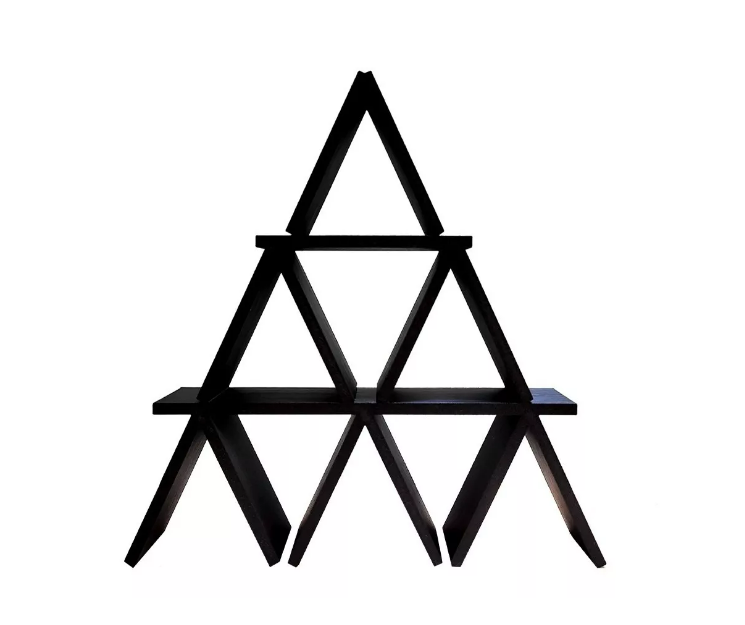
\includegraphics[scale=0.4]{lampada/piramide.png}
\end{center}

\subsection*{Entrada}
A entrada possui somente uma linha e contém a altura $h$ ($1 \leq h \leq 10^9$) da pirâmide que Aladdin precisa montar.

\subsection*{Saída}
Imprima 1 linha com a quantidade de cartas necessárias para montar uma pirâmide de altura $h$.

\begin{table}[!h]
\centering
\begin{tabular}{|l|l|}
\hline
\begin{minipage}[t]{3in}
\textbf{Exemplo de entrada}
\begin{verbatim}
1
\end{verbatim}
\vspace{1mm}
\end{minipage}
&
\begin{minipage}[t]{3in}
\textbf{Exemplo de saída}
\begin{verbatim}
2
\end{verbatim}
\vspace{1mm}
\end{minipage} \\
\hline
\end{tabular}
\end{table}
\begin{table}[!h]
\centering
\begin{tabular}{|l|l|}
\hline
\begin{minipage}[t]{3in}
\textbf{Exemplo de entrada}
\begin{verbatim}
10
\end{verbatim}
\vspace{1mm}
\end{minipage}
&
\begin{minipage}[t]{3in}
\textbf{Exemplo de saída}
\begin{verbatim}
155
\end{verbatim}
\vspace{1mm}
\end{minipage} \\
\hline
\end{tabular}
\end{table}
